\documentclass[UTF8]{ctexart}[a4paper,10pt]
\usepackage[thmmarks]{ntheorem}
\usepackage{amsmath}
\usepackage{amsfonts,amssymb} 
\usepackage{thmtools}
\usepackage[hmargin=2.5cm,vmargin=2.5cm]{geometry}
\usepackage{tikz-cd,tikz}
\usepackage{graphicx,float}
\usepackage{fancyhdr}
\usepackage{fourier-orns}
\usepackage{quiver}
\usepackage{subfigure}
%声明环境
\newtheorem{example}{例}[subsection]              
\newtheorem{algorithm}{算法}[subsection]
\newtheorem{theorem}{定理}[subsection]            
\newtheorem{definition}{定义}[subsection]
\newtheorem{axiom}{公理}[subsection]
\newtheorem{proXperty}{性质}[subsection]
\newtheorem{proposition}{命题}[subsection]
\newtheorem{lemma}[theorem]{引理}
\newtheorem{corollary}[theorem]{推论}
{
    \theoremheaderfont{\sffamily}
    \newtheorem*{remark}{注解} 
}
\newtheorem{condition}{条件}[subsection]
\newtheorem{conclusion}{结论}[subsection]
\newtheorem{assumption}{假设}[subsection]
{
\theoremstyle{nonumberplain}
\theoremheaderfont{\bfseries}
\theorembodyfont{\normalfont}
\theoremsymbol{\mbox{$\Box$}}
\newtheorem{proof}{证明}
}
%定义命令
\def\N{\mathbb{N}}
\def\Z{\mathbb{Z}}
\def\Q{\mathbb{Q}}
\def\R{\mathbb{R}}
\def\C{\mathbb{C}}
\def\S{\mathbb{S}}
\def\D{\mathbb{D}}
\def\H{\mathbb{H}}
\def\cC{\mathcal{C}}
\def\cD{\mathcal{D}}

%页眉设计
\renewcommand 
\headrule{
\hrulefill
\raisebox{-2.1pt}
{\quad{\FourierOrns M T S N}\quad}
\hrulefill}
\pagestyle{fancy}

%极限、余极限与滤过余极限的实现
\makeatletter
\newcommand{\Colim@}[2]{
  \vtop{\m@th\ialign{##\cr
    \hfil$#1\operator@font lim$\hfil\cr
    \noalign{\nointerlineskip\kern1.5\ex@}#2\cr
    \noalign{\nointerlineskip\kern-\ex@}\cr}}%
}
\newcommand{\Colim}{%
  \mathop{\mathpalette\Colim@{\rightarrowfill@\scriptscriptstyle}}\nmlimits@
}
\makeatother

\makeatletter
\newcommand{\Lim@}[2]{%
  \vtop{\m@th\ialign{##\cr
    \hfil$#1\operator@font lim$\hfil\cr
    \noalign{\nointerlineskip\kern1.5\ex@}#2\cr
    \noalign{\nointerlineskip\kern-\ex@}\cr}}%
}
\newcommand{\Lim}{%
  \mathop{\mathpalette\Lim@{\leftarrowfill@\scriptscriptstyle}}\nmlimits@
}
\makeatother


\makeatletter
\newcommand{\colim@}[2]{%
  \vtop{\m@th\ialign{##\cr
    \hfil$#1\operator@font oli~$\hfil \cr
    \noalign{\nointerlineskip\kern1.5\ex@}#2\cr
    \noalign{\nointerlineskip\kern-\ex@}\cr}}%
}
\newcommand{\colim}{%
  \mathop{\mathrm{c}\mathpalette\colim@{\rightarrowfill@\scriptscriptstyle}\mathrm{\!\!m}}\nmlimits@
}
\makeatother

\makeatletter
\newcommand{\cone@}[1]{%
  \vtop{\m@th\ialign{##\cr
    \hfil$#1\operator@font cone$\hfil\cr
    \noalign{\nointerlineskip\kern1.5\ex@}\cr
    \noalign{\nointerlineskip\kern-\ex@}\cr}}%
}
\newcommand{\cone}{%
  \mathop{\mathpalette\cone@{\scriptscriptstyle}}\nmlimits@
}
\makeatother
%超链接红色
\usepackage[colorlinks,linkcolor=red]{hyperref}

\usepackage{enumerate}


\title{2023年春数论课程笔记}
\author{整理者:子綦·子游}
\begin{document}
\maketitle
\tableofcontents
\section{授课老师信息}
名字:栗慧曦

办公室:数院414

分为:初等数论 解析数论 代数数论 

网课推荐: Core Topics in Modern number theory 
\section{初等数论}
以下事实将被默认:
\begin{proposition}[良序原理]
    任何非空的正整数集合都包含一个最小的元素。
\end{proposition}
\begin{corollary}
    数$\sqrt{5}$不是有理数。
\end{corollary}
\begin{proof}
    考虑$S=\{b:b \in \Z_{+}, there \quad exists\quad an \quad integral\quad a \quad such \quad that \quad \dfrac{a}{b}=\sqrt{5}\}$。我们假定$S$非空。则根据良序原理,$S$有最小的元素$y$,设$\dfrac{x}{y}=\sqrt{5}$,$x \in \Z$.

    于是$x^2=5y^2$。$x^2-2xy=5y^2-2xy$,$x(x-2y)=y(5y-2x)$.于是$\dfrac{x}{y}=\dfrac{5y-2x}{x-2y}$。

    显然$x-2y=(\sqrt{5}-2)y>0$,并且$x-2y<y$,$\sqrt{5}<3$。于是矛盾于$y$最小!因此$S$是空集,这意味着$\sqrt{5}$是无理数。
\end{proof}
\subsection{费马-欧拉定理及其应用}
\begin{theorem}[费马-欧拉]
    设$a,n$是两个互素的正整数,即$(a,n)=1$。那么下式成立:
    $$
    a^{\varphi(n)}\equiv 1(\mathrm{mod}  n)
    $$
\end{theorem}
\begin{proof}
    考虑群$\Z/n \Z$有阶数$\varphi(n)$,证毕。
\end{proof}
\begin{example}
    $2^{12} \equiv 1 (\mathrm{mod}13)$。
     
    $3^6 \equiv 1 (\mathrm{mod}14)$。
\end{example}
\begin{corollary}[费马小定理]
    给定一个素数$p$和一个整数$a$,且$(a,p)$互素。则$a^{p-1} \equiv 1(\mathrm{mod} p)$。
\end{corollary}
\begin{corollary}[费马小定理·形式2]
    设$p$是一个素数,则$a^p \equiv a (\mathrm{mod} p)$。
\end{corollary}
 
 对于一个较大的奇整数$n$,若$2^n$模$n$不等于$2$,则$n$是一个合数。这一点可以用于判定一个数是否是素数。这被称为Fermat's primality test to base 2.

 素数是正整数,且必须严格大于1.这一点很容易搞错。

 判定一个数是否是素数,如果使用蛮力计算,事实上可以在$C \sqrt{n}$步内计算$n$的素因数分解。而Fermat's primality test 仅需要O$(log(n))$步。



 \begin{definition}
    如果一个数$n$能够通过所有的费马素数测试法,则称其为\rm{Carmichael}数。事实上,Carmichael数的个数是无穷多个。
 \end{definition}

 我们继续介绍Miller test方法来判定一个数是否是素数。

 对于奇数$n$,我们首先将$n-1$写为$2^rs$,$r \geq 1$,$s$是一个基数。我们验证$a^s \equiv 1(\mathrm{mod}n)$,$a^s \equiv -1 (\mathrm{mod}n) ,\dots, a^{2^{r-1}s}\equiv -1(\mathrm{mod}n)$

 如果都不成立,则$n$是一个合数。

 如果合数$n$通过了Miller测试,说明其伪装的很好。我们称之为在底$a$下的强pseudoprime(伪素数)。

\begin{example}
  对$25$使用$2$为基的Miller测试:
  
  $25-1=2^3 \times 3$.$2^3 \equiv 8$,$2^{2 \times 3}\equiv 14$,$2^{2^2 \times 3} \equiv 21$。所以$25$未通过,是合数。
\end{example}
\begin{remark}
  一个合数至多能通过$1/4$的Miller测试。因而如果一个数通过了很多底的Miller测试,从概率上讲其非常可能是一个素数。比如,若其通过了$10$个测试,则不是素数的可能性仅为$(1/4)^10$。
\end{remark}
\subsection{中国剩余定理}
\begin{proposition}
  方程$ax \equiv b \quad (\mathrm{mod m})$是可解的,当且仅当$d|b$,其中$d=(a,m)$.当$d|b$,方程有$d$个不同的解:
  $$
  x_0,x_0+m/d,\dots,x_0+(d-1)m/d
  $$

\end{proposition}
\begin{theorem}[CRT]
    设$m_1,\dots,m_s$是两两互素的,其中$s\geq 2$.假设$(a_i,m_i)=1$,$1 \leq i \leq s$,那么方程组:
     $$
     a_ix \equiv b_1 (\mathrm{mod}\quad  m_i)
     $$
     在$\mathrm{mod} M=m_1 \dots m_n$的要求下具有唯一的解。
\end{theorem}
\begin{proof}
  定理的证明充满着比较繁琐的构造。这里省略。但是为了解方程,又不得不说明怎么来的。因此我直接截取讲义的一部分:
  \begin{figure}[htpb]
    \centering
    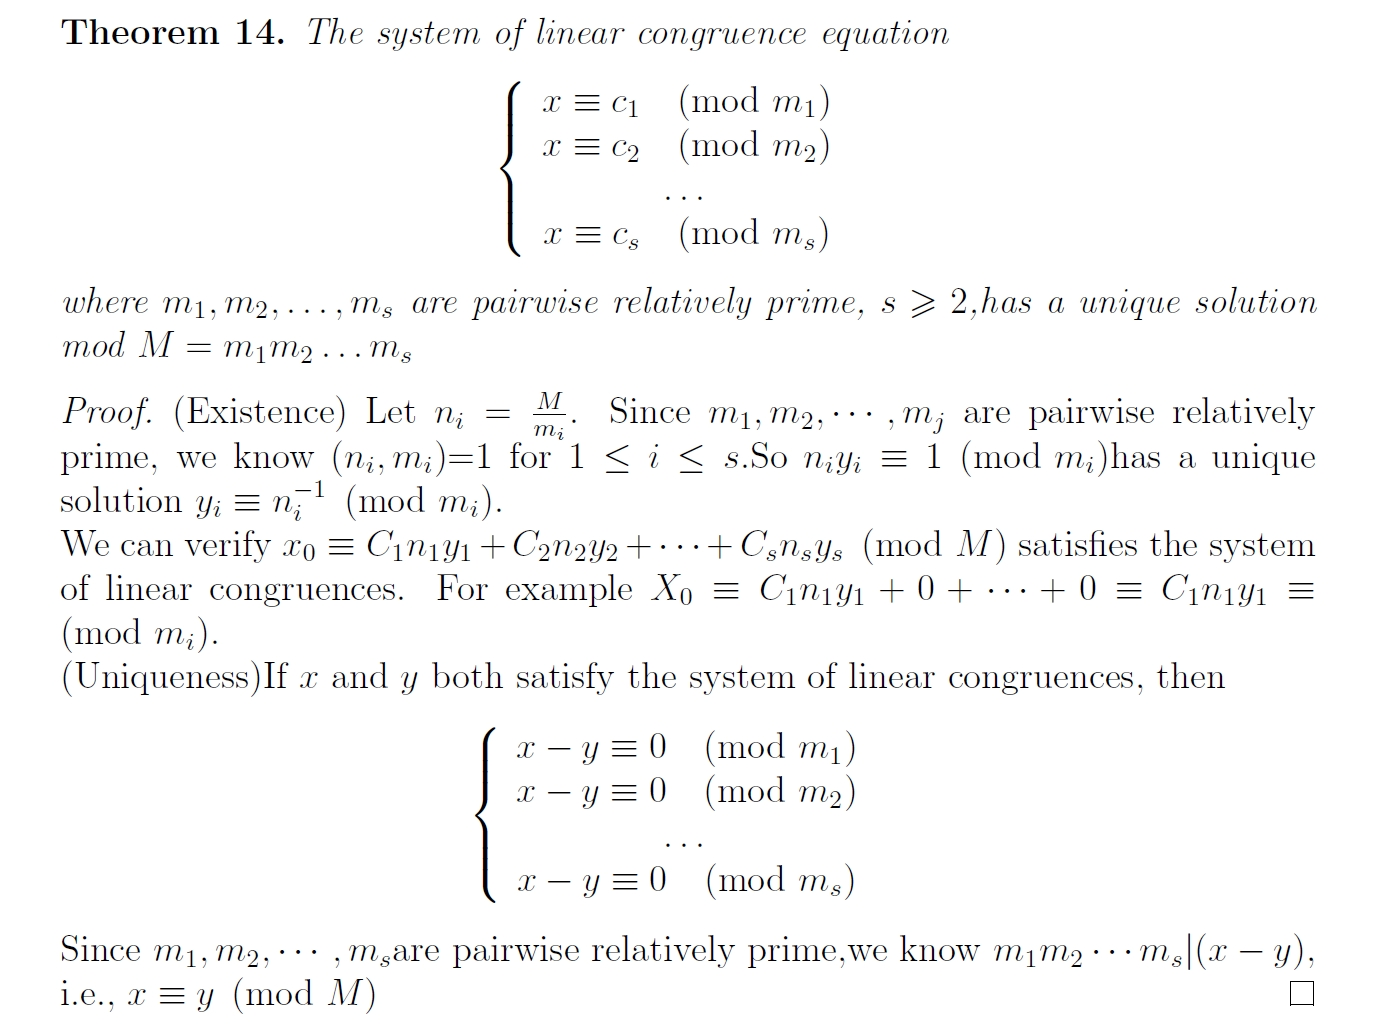
\includegraphics[scale=0.3]{CRT.jpeg
    }
  \end{figure}
\end{proof}
\section{代数数论}
\begin{definition}
  设正整数$a,b,c$满足:
  \begin{align}
    a^2+b^2=c^2 \quad (a,b,c)=1
  \end{align}
  则称$(a,b,c)$是互素的毕达哥拉斯三元数组。
\end{definition}
  \begin{theorem}
    $(a,b,c)$是互素的毕达哥拉斯三元数组,则存在一个偶数且:
    \begin{align}
      a=2st,\ b=t^2-s^2,\ c=t^2+s^2, \mathrm{where}\ 0<s<t,\ (s,t)=1
    \end{align}
    使得$s,t$一奇数一偶数。
  \end{theorem}
  \begin{proof}
    $a^2=c^2-b^2$,于是:
    \begin{align}
      (a/2)^2=(c+d)/2(c-d)/2
    \end{align}
    我们断言$\dfrac{c+d}{2}$和$\dfrac{c-d}{2}$都是平方数。若不然,则两者有公共的素因子。显然不能是$2$,则$c$和$b$不互素。

    设$t^2=\dfrac{c+d}{2}$,$s^2=\dfrac{c-d}{2}$。显然$s<t$且$(s,t)=1$。且$s,t$之中一奇数一偶数。

    若$a,b,c$满足等式。我们只需要验证$(a,b,c)$互素。这也是显然的。
    \end{proof}
    费马大定理说明当$n\geq 3$的时候,上述方程没有非平凡的整数解。我们之后将会证明:$n=3$时,$x^3+y^3=z^3$没有非平凡的解,其中$x,y,z \in \Z[\dfrac{-1+\sqrt{-3}}{2}]$
   \begin{proposition}
    方程$x^4+y^4=z^2$没有非平凡的解。
   \end{proposition}
   \begin{proof}
      显然不妨设$(x,y)=1$。我们考虑$x^4+y^4=z^2$。此时$(x^2,y^2,z)$是毕达哥拉斯互素的三元对。于是存在$0<n<m$一奇数一偶数满足:$x^2=2mn,y^2=m^2-n^2,z=m^2+n^2$。

      如果$m$是偶数,$n$是奇数,则$y^2$模$4$余$3$。矛盾!

      于是$n^2+y^2=m^2$。于是$m=a^2$,$a$是奇数。$2n=b$,$b$是偶数。设$b=2c$,则$n=2c^2$。于是:
      \begin{align}
        a^4=m^2=n^2+y^2=4c^2+y^2
      \end{align}
      因此$(2c^2,y,a^2)$是毕达哥拉斯互素的三元对。因此:
      \begin{align}
        2c^2=2m_1n_1 \quad y=m_1^2-n_1^2 \quad a^2=m_1^2+n_1^2 \dots
      \end{align}
      因此$m_1=a_1^2$,$n_1=b_1^2$.此时$a^2=a_1^4+b_1^4$。因此$(a_1,b_1,a)$也是一个非平凡的解$x^4+y^4=z^2$。但是$z=m^2+n^2>a\dots$。根据良序引理容易导出矛盾。
   \end{proof}
   为了证明费马最后一个定理,我们只需要说明$x^p+y^p=z^p$,$p$是一个素数。我们考虑$p=3$的情况,但是此时$x,y,z \in \Z[\dfrac{-1+\sqrt{-3}}{2}]$.
   \begin{definition}
    一个复数$\xi$被称为一个代数数,若存在一个首项为$1$的多项式$f(x)\in \Z[x]$使得$f(\xi)=0$。
   \end{definition}
   \begin{theorem}
    $\Q$中的代数数只有$\Z$。
   \end{theorem}
   我们称$K/\Q$是一个数域,若$[K:Q]<\infty$。我们用$\mathcal{O}_K$表示所有的$K$中的代数数。则$\mathcal{O}_{\Q}=\Z$。

   我们将会关心$K=\Q[\sqrt{-m}]$其中$m$是一个正的非平方数。根据抽象代数的知识,我们有:
   \begin{align}
    \mathcal{O}_{\Q[\sqrt{-m}]}=\Z[-\sqrt{-m}], m\equiv 1(\mod 4);=\Z[\dfrac{1+\sqrt{-m}}{2}], m\equiv 3(\mod 3)
   \end{align}

   定义映射$N$:
   \begin{align}
    N:\mathcal{O}_{\Q[\sqrt{-m}]} \to \Z \quad ; a+b\sqrt{-m} \mapsto a^2+mb^2 \ a,b \in \Q
   \end{align}
   可以验证$N(ab)=N(a)N(b)$.$N(a)=0$当且仅当$a=0$。$N(a)=1$当且仅当$a$是一个单位。
   \begin{proposition}
    整环$\mathcal{O}_{\Q[\sqrt{-3}]}=\Z[\dfrac{1+\sqrt{-3}}{2}]$是一个欧几里得环,即我们可以在环里面做带余除法。
  \end{proposition}
    \begin{lemma}
      设$\alpha \in \mathcal{O}_{\Q[-\sqrt{3}]}$。若$N(\alpha)$是一个有理素数则$\alpha$是$\mathcal{O}_{\Q[\sqrt{-3}]}$上的素元。
    \end{lemma}
    \begin{proof}
      显然。
    \end{proof}
    \begin{corollary}
      考虑$N(\sqrt{-3})=3$是$\Z$中的素数,则$\sqrt{-3}$是素元素。
    \end{corollary}
   接下来我们考虑方程$x^3+y^3=z^3$在模$\sqrt{-3}$下的解。$\sqrt{-3}$的伴随是$\sqrt{-3}$,$-\sqrt{-3}$,$\omega-1$,$\dots$.
\end{document}